% ============================================================================
\section{Testing the formulas and cross-validating with The Virtual Brain}
\label{sec:twin}

The request was to build simulations using the derived formulas and one using an existing real simulator, and to compare them (\code{infer.py}, \code{tvb_compare.py}).

\subsection{Method: twin experiments with deliberate confounds}

In a twin experiment a simulator with known hidden values synthesises the signal a sensor would record, realistic confounds are added, the inference method is applied, and the result is compared with the truth. Confounds are essential; otherwise inverting the same equation is trivially perfect.

\begin{table}[H]
\centering\small
\caption{Confounds injected in the twin experiments.}
\begin{tabularx}{\linewidth}{@{}l l l L@{}}
\toprule
Confound & Used in & Value & Realism \\
\midrule
Glial slope unknown & E1 & true 51 vs textbook 61.5 mV/decade & Measured mammalian glia \\
Skull attenuation unknown & E2 & true $\alpha=0.01$, guessed 0.005 & Cortex-to-scalp gain varies \\
Electrode drift & E2 & random walk 0.4 \uV/step & DC-EEG's main practical problem \\
\EGABA{} estimation error & E3 & $\pm$2 mV & TMS-EEG estimates are indirect \\
\HCO/\Clm{} permeability & E3 & $r$ = 0.2--0.44 & Literature range \\
Scalp haemodynamics & E5 & Mayer waves 0.1 Hz + cardiac 1.2 Hz & Dominant fNIRS contaminant \\
Partial volume & E5 & 15\% of photon path in cortex & Layered head \\
Individual DPF & E5 & true DPF 10\% above formula & Inter-subject variation \\
Onset-picking noise & T2 & $\pm$20 ms & SEEG annotation \\
\bottomrule
\end{tabularx}
\end{table}

\subsection{Results E1--E7}

\paragraph{E1: \Kp{} from a glial electrode.} Textbook slope (61.54): RMSE 0.239\,mM, peak 10.29\,mM (true 12.21, $-16$\%). Measured slope (51): RMSE \textbf{0.062}\,mM, peak 12.32\,mM (+1\%). The inverse is exact only with the measured slope.

\paragraph{E2: \Kp{} from scalp DC-EEG with a Kalman filter.} The process model $d[\mathrm K]_o/dt = a\cdot\mathrm{rate} - ([\mathrm K]_o - K_0)/\tau$ was calibrated on healthy data ($a=0.093$, $\tau=0.51$\,s) and applied to epileptic data whose clearance is 3$\times$ slower. Naive constant-gain conversion: RMSE 1.41\,mM, peak \textbf{29.2}\,mM (2.4$\times$ too high). Activity-driven process model alone: 0.51\,mM (peak 14.1). EKF (process model + DC): \textbf{0.50}\,mM (peak 14.0); the EKF's skull-gain estimate was 0.015 (true 0.010). Honest finding: with unknown gain and drift the DC channel added almost nothing beyond the EEG-driven model; it would need a calibrated gain.

\paragraph{E3: \Cli{} from an \EGABA{} estimate.} Chord inverse: RMSE \textbf{1.12}\,mM, bias $-0.13$. GHK: $r=0.20$ RMSE 3.05 (bias \textbf{+2.72}); $r=0.25$ 2.50 (+2.09); $r=0.44$ 1.47 ($-0.32$, a coincidental crossing). With the right formula $\pm$2\,mV of \EGABA{} error becomes $\approx\pm$1.1\,mM, enough to separate healthy (5.6) from epileptic (11.6) tissue; the wrong formula family adds a systematic bias up to 2.7\,mM.

\paragraph{E4: E/I from the EEG spectrum.} 30--50\,Hz fixed fit: $\chi$ = 1.65 healthy ($R^2$ 0.87) vs 1.50 epileptic (0.75), the direction associated with more excitation. The broadband 2--200\,Hz knee fit failed in epileptic tissue ($\chi\approx0$, $R^2$ 0.74) because interictal spikes inject high-frequency power. $\chi$ is usable only as a relative marker, in a narrow band and outside bursts.

\paragraph{E5: HbO/HbR from fNIRS.} Naive MBLL: RMSE 10.3\,\uM, correlation 0.873, amplitude 22\%. With short-channel regression: correlation \textbf{0.996}, amplitude 16\%. With partial-volume correction: RMSE \textbf{1.40}\,\uM, amplitude 1.10 (the residual +10\% is exactly the injected DPF error). HbR, full pipeline: 0.49\,\uM, r = 0.999. A Temple-style device without a short channel and depth information would underestimate cortical flow about 5$\times$ and be contaminated by scalp physiology.

\paragraph{E6: adenosine from postictal silence.} $A_{peak}e^{-T/20}$ reproduced the true adenosine at recovery in both tissues (0.060 vs 0.061 healthy; 0.195 vs 0.196 epileptic), so the decay law is exact, but the level at which firing resumes differs 3.2$\times$ between tissues; a universal threshold does not exist, confirming the withdrawal.

\paragraph{E7: KCC2 strength by Bayesian grid inference.} Observed features: resting \EGABA{} ($\pm$1.5\,mV) and mean excitatory rate ($\pm$25\%); six ionic runs at different KCC2 strengths.

\begin{table}[H]
\centering\small
\caption{E7: posterior over KCC2 strength (true 0.3).}
\begin{tabular}{@{}lcccccc@{}}
\toprule
KCC2 ($\times$ normal) & 0.15 & 0.2 & \textbf{0.3} & 0.45 & 0.7 & 1.0 \\
\midrule
Simulated \EGABA{} (mV) & $-51.3$ & $-52.5$ & $-54.2$ & $-56.4$ & $-60.7$ & $-63.5$ \\
Simulated E rate (Hz) & 13.2 & 12.4 & 9.9 & 12.2 & 10.3 & 10.9 \\
Posterior & 0.014 & 0.103 & \textbf{0.414} & \textbf{0.468} & 0.001 & $\approx$0 \\
\bottomrule
\end{tabular}
\end{table}

Posterior mean \textbf{0.36$\pm$0.09} (true 0.30); the MAP fell on 0.45 because the noisy \EGABA{} ``measurement'' was $-55.3$ vs $-54.0$\,mV. \EGABA{} carries almost all the information (rate is non-monotonic in KCC2); healthy and severe-loss values are correctly ruled out, 0.3 vs 0.45 honestly not.

\begin{figure}[H]
\centering
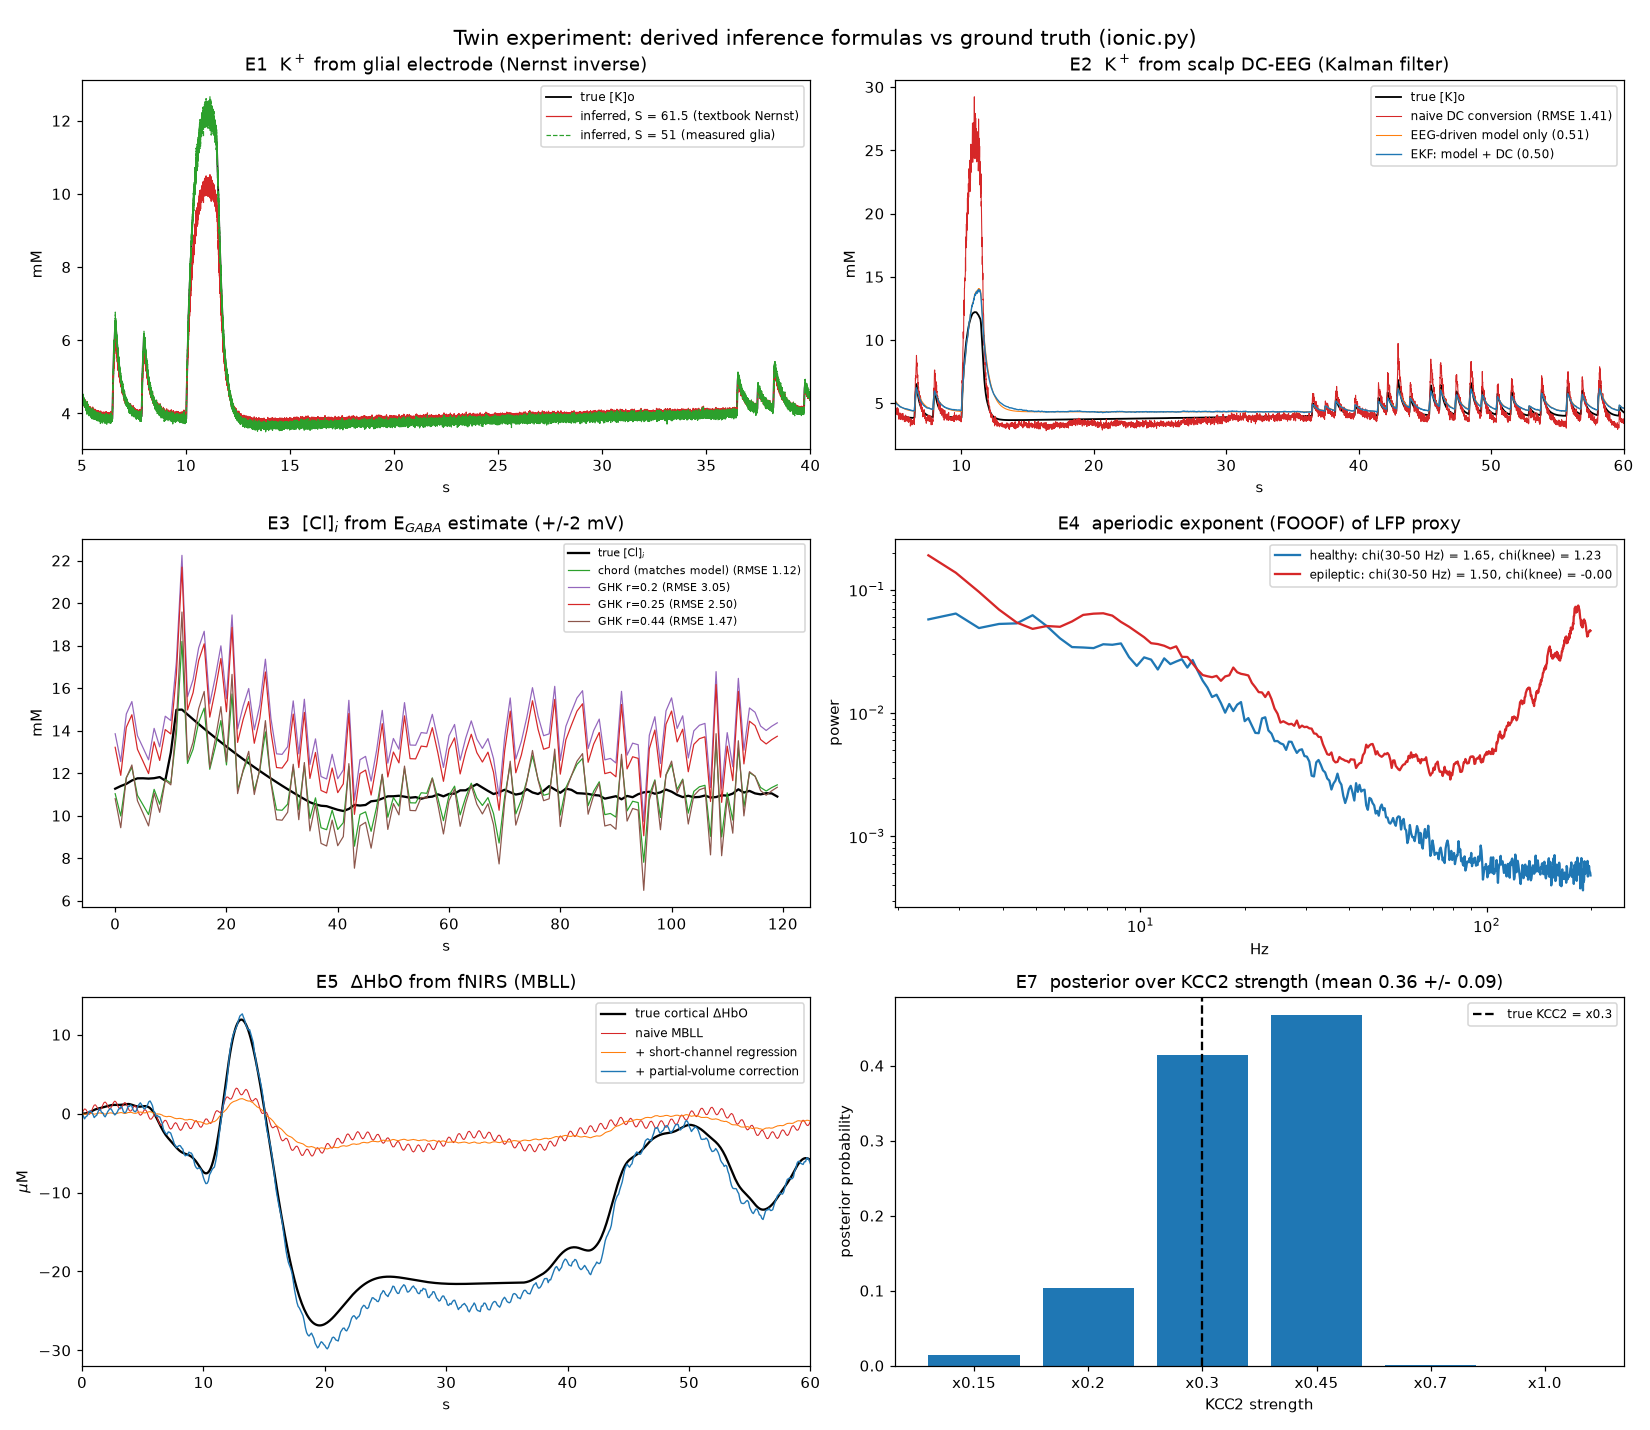
\includegraphics[width=0.85\linewidth]{epilepsy_sim/output/infer_results.png}
\caption{Twin experiments E1--E7.}
\end{figure}

\subsection{The Virtual Brain}
\label{sec:tvb}

\paragraph{T1: our Epileptor vs TVB's official Epileptor.} Same equations (checked line by line against TVB's source), parameters ($x_0=-1.6$, $I_{ext}=3.1$, $r=1/2857$) and initial state.

\begin{table}[H]
\centering\small
\caption{T1 cross-validation.}
\begin{tabular}{@{}llll@{}}
\toprule
& TVB (Heun, dt 0.05) & Ours (Euler, dt 0.05) & Ours (Euler, dt 0.01) \\
\midrule
Seizures in 6000 a.u. & 3 & 3 & 3 \\
Onsets & 886.2, 2820.2, 4754.2 & 887.0, 2883.0, 4880.0 & \textbf{886.2}, 2827.6, 4769.0 \\
Seizure duration & 968.7 & 1030 & \textbf{976.2} \\
$z$ RMSE vs TVB & -- & 0.139 & \textbf{0.018} \\
LFP correlation & -- & 0.71 & 0.87 \\
Runtime & 43 s & 1.5 s & 6.4 s \\
\bottomrule
\end{tabular}
\end{table}

The first onset is identical and all differences shrink with the time step, so they come from the integrator (Euler vs Heun), not the model: \code{main.py}'s Epileptor is validated and 7--30$\times$ faster for one region.

\paragraph{T2: VEP-style whole-brain inference.} TVB's 76-region connectome (3\,m/s conduction, Difference coupling $a=1$, permittivity coupling $K_s=-0.2$), epileptogenic zone rAMYG ($x_0=-1.6$), propagation zone rPHC, rTCV, rTCPOL ($-2.0$), all others $-2.2$. The EZ seized first (onset 1022\,ms, recurring $\approx$1.4\,s) and the seizure spread to \textbf{36 of 38} right-hemisphere regions and none on the left. From onset times alone ($\pm$20\,ms noise), the EZ was localised correctly and its excitability recovered as $-1.60\pm0.0002$ (posterior $8\times10^{-8}$ at $-1.7$, $3\times10^{-6}$ at $-1.5$). This is an \textbf{inverse crime}: the same model, parameters and grid (containing the exact truth) generated and fitted the data, so the posterior collapses unrealistically; real SEEG with model mismatch widens uncertainty a lot. E7, by contrast, shows honest uncertainty.

\begin{figure}[H]
\centering
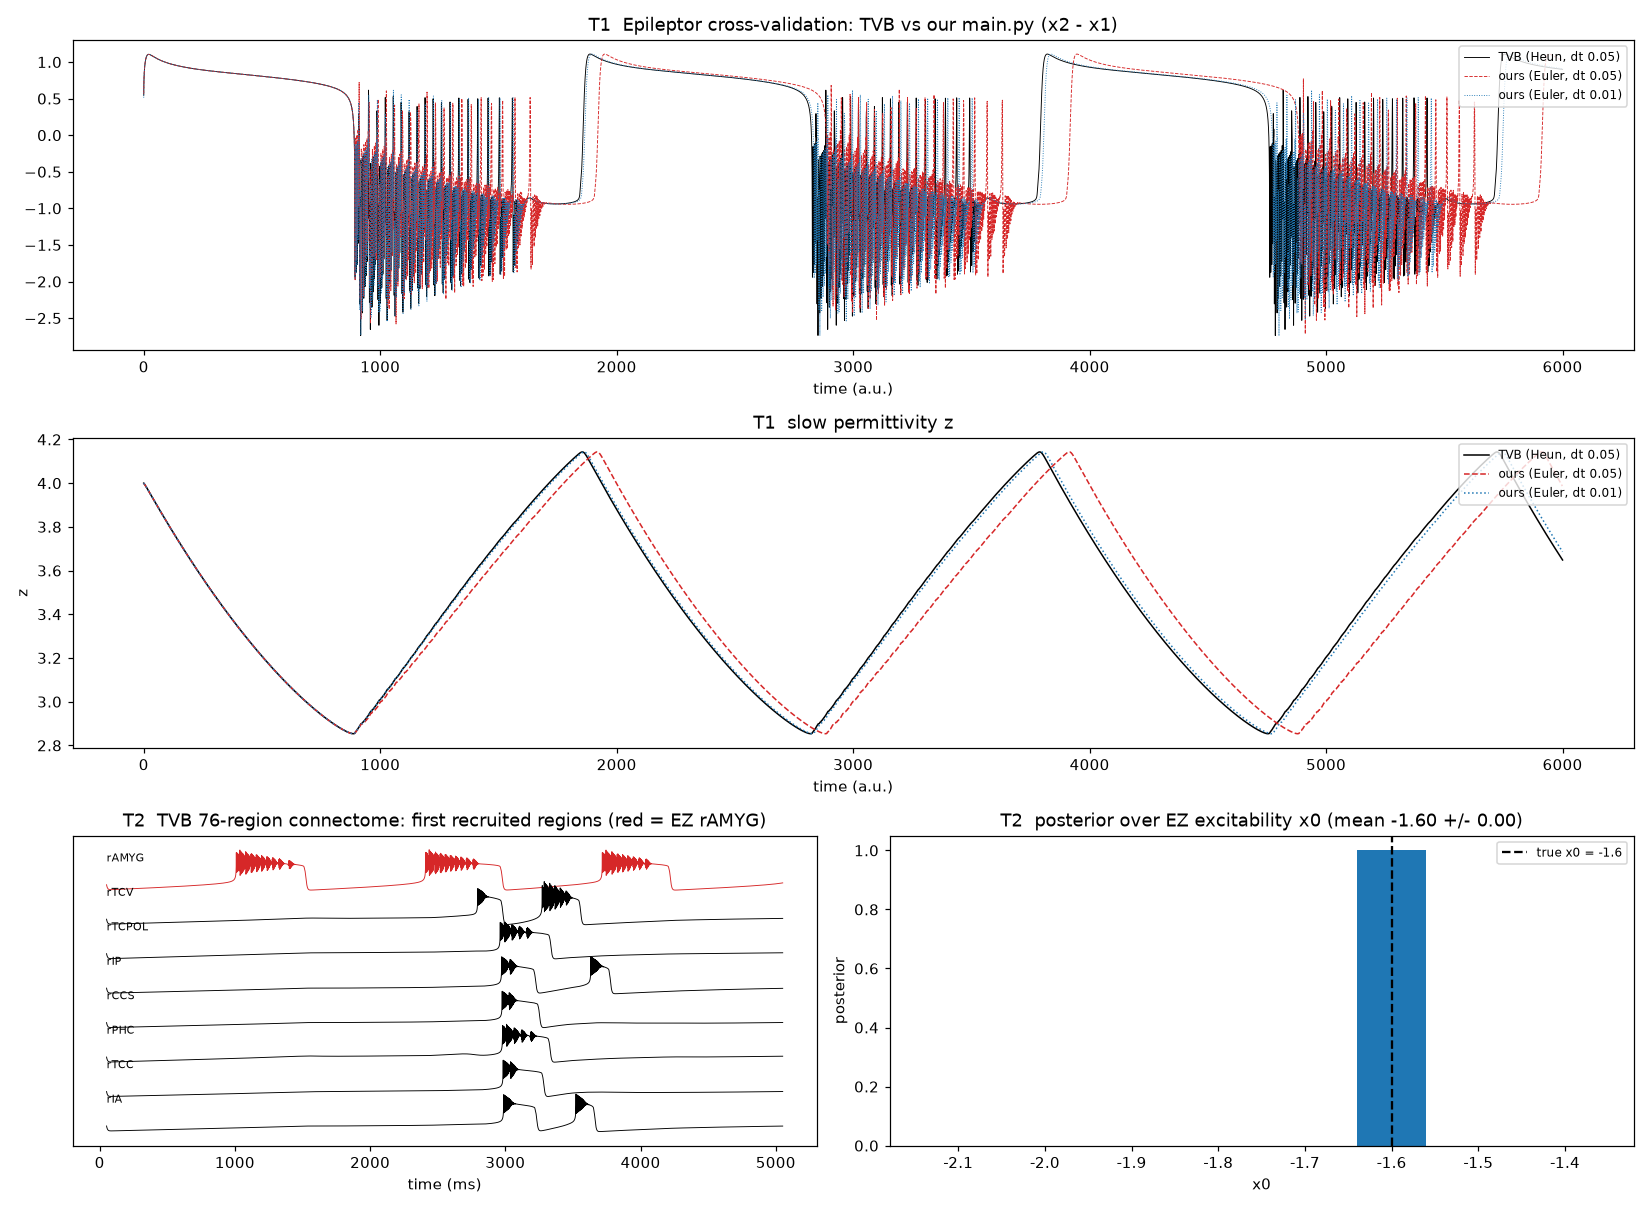
\includegraphics[width=0.85\linewidth]{epilepsy_sim/output/tvb_compare.png}
\caption{TVB cross-validation (T1) and VEP-style inference (T2).}
\end{figure}

\subsection{Head-to-head and conclusions}

Our ionic model is biophysical, local ($\approx$1\,mm\textsuperscript{2}), infers ions in physical units and answers \emph{why} tissue is epileptic; TVB is phenomenological, whole-brain, localises and propagates seizures and answers \emph{where}. They are complementary: TVB would locate the epileptogenic zone, \code{ionic.py} fitted to that region's EEG, TMS-EEG and fNIRS would infer the mechanism (KCC2 vs glia vs clearance), and the ionic pathology could be mapped back onto TVB's $x_0$ (the Epileptor-2 motivation of Chizhov et al.\ 2018). Overall: derived formulas work when their assumptions hold and fail exactly as predicted when they do not (textbook slope $-16$\%, naive DC 2.4$\times$, GHK bias +2.7\,mM, naive fNIRS 22\% amplitude); model-based inference beats single-formula conversion; some variables (adenosine, KCC2) need the full model; and the code is validated twice (Cressman and TVB).
